\documentclass[10pt,conference,onecolumn,compsoc]{IEEEtran}


\usepackage{hyperref}
\usepackage{enumitem}
\setlist[itemize]{leftmargin=3 cm}
\setlist[enumerate]{leftmargin=3cm}



% *** CITATION PACKAGES ***
%
\ifCLASSOPTIONcompsoc
  % IEEE Computer Society needs nocompress option
  % requires cite.sty v4.0 or later (November 2003)
  \usepackage[nocompress]{cite}
\else
  % normal IEEE
  \usepackage{cite}
\fi

% *** GRAPHICS RELATED PACKAGES ***
%
\ifCLASSINFOpdf
   \usepackage[pdftex]{graphicx}
  % declare the path(s) where your graphic files are
  % \graphicspath{{../pdf/}{../jpeg/}}
  % and their extensions so you won't have to specify these with
  % every instance of \includegraphics
  % \DeclareGraphicsExtensions{.pdf,.jpeg,.png}
\else
  % or other class option (dvipsone, dvipdf, if not using dvips). graphicx
  % will default to the driver specified in the system graphics.cfg if no
  % driver is specified.
  % \usepackage[dvips]{graphicx}
  % declare the path(s) where your graphic files are
  % \graphicspath{{../eps/}}
  % and their extensions so you won't have to specify these with
  % every instance of \includegraphics
  % \DeclareGraphicsExtensions{.eps}
\fi




% correct bad hyphenation here
\hyphenation{op-tical net-works semi-conduc-tor}


\begin{document}

\title{SBI Managment system}


\author{Kevin Patel\\Jeff Jordan
}

\IEEEtitleabstractindextext{%
\begin{abstract}
SBI Management System, named after the flagship Stone Brook Inn, is a program for use in the commercial Hospitality business in order to easily navigate the processes of booking, reserving, and maintaining rooms in an effective way to alleviate stresses of overbooking and unavailable rooms within businesses. 

\end{abstract}
}
\maketitle

\IEEEdisplaynontitleabstractindextext

\IEEEpeerreviewmaketitle



\section{Introduction}

The purpose of the SBI Management system is to remove the clerical errors of record keeping by hand and to cut down on the potential mistakes that could happen with note taking with rotating cast of
managerial staff and employees. It is designed around the idea of condensing and centralizing all reservation and booking information into one simple, easy-to-use application in order to remove the stress of record keeping and room tracking. 

On the backend, it will keep track of non-confidential customer information. The purpose of this is to implement features such as a customer rewards program, discounts, personalized service, etc. In the future, it will implement encryption for payment information. 

\subsection{Background}
A member of our group's family owns a hotel. This project is being designed with the needs of an actual hotel business in mind. The design will be centered around a simple GUI to quickly assign rooms and check availability. 

While the primary purpose of the project is for the Stone Brook Inn, we will design it to be implemented by any local small hotel or motel. The idea is to keep the functionality universal while making design edits simple and easy to understand. 

\subsection{Challenges}
Integrating legal and secure encryption for web payments will be the ultimate challenge for the project. 
Ensuring that the program doesn't allow for any booking of unavailable rooms will be a challenge since there will be a lot of test cases that might go unnoticed.
Designing a universal program that could be adjusted to fit any business model might present itself to be more challenging than we can currently foresee. 


\section{Scope}
The scope of this program will be extensive. It will handle guest checkins and checkouts, it will feature an intuitive and powerful interface, it will be adjustable to any hotel, it will ensure no overbooking issues arise, will keep track of customer rewards points, and lastly, feature a cross-shift note system. 

\subsection{Requirements}
As part of fleshing out the scope of your requirements, you'll also need to keep in mind both your functional and non-functional requirements.  These should be listed, and explained in detail as necessary.  Use this area to explain how you gathered these requirements.

\subsubsection{Functional}
\begin{itemize}
\item User needs to have a private shopping cart -- this cannot be shared between users, and needs to maintain state across subsequent visits to the site
\item Users need to have website accounts -- this will help track recent purchases, keep shopping cart records, etc.
\item You'll need more than 2 of these...
\end{itemize}

\subsubsection{Non-Functional}
\begin{itemize}
\item Security -- user credentials must be encrypted on disk, users should be able to reset their passwords if forgotten
\item you'll typically have fewer non-functional than functional requirements
\end{itemize}

\subsection{Use Cases}

\begin{table}
\centering
\begin{tabular}{|c|c|c|c|c|}
\hline
1 & Release occupancy\\
\hline \hline
2 & Fill vacancy\\
\hline

\end{tabular}
\caption{Use Cases}
\label{tab:useCaseIndex}
\end{table}


\begin{itemize}
\item[Use Case Number:] 1
\item[Use Case Name:] Booking and Maintaining Rooms
\item[Description:] Administrators at motel and hotel businesses will be able to block rooms once they are booked by customers or repairs/cleaning needs to take place.

\item[Use Case Number:] 2
\item[Use Case Name:] Reservations
\item[Description:] Interact with a calender in order to properly plan out and schedule rooms to be booked and blocked to prevent overbooking.
\end{itemize}

\begin{itemize}
\item[Use Case Number:] 2
\item[Use Case Name:] Checkout
\item[Description:] A shopper on our site has finished shopping.  They will click on a ``Checkout" button.  This will kick off a process to calculate cart total, any taxes, shipping rates, and collect payment from the shopper.

\end{itemize}

You will then need to continue to flesh out all use cases you have identified for your project.



\subsection{Interface Mockups}
\begin{figure}[ht!]
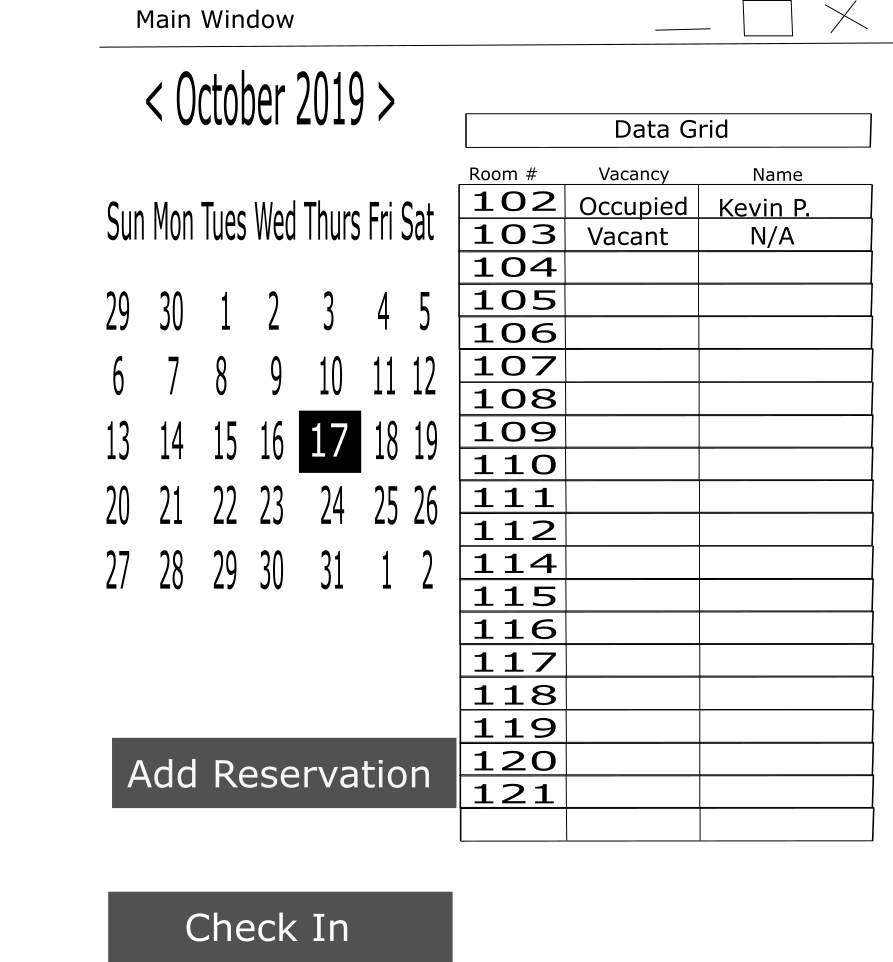
\includegraphics[height=250px, width=350px]{MainWindowGUI.png}
\caption{Main window of the program}
\label{Interface}
\end{figure}

\subsection{Interface Mockups}
\begin{figure}[ht!]
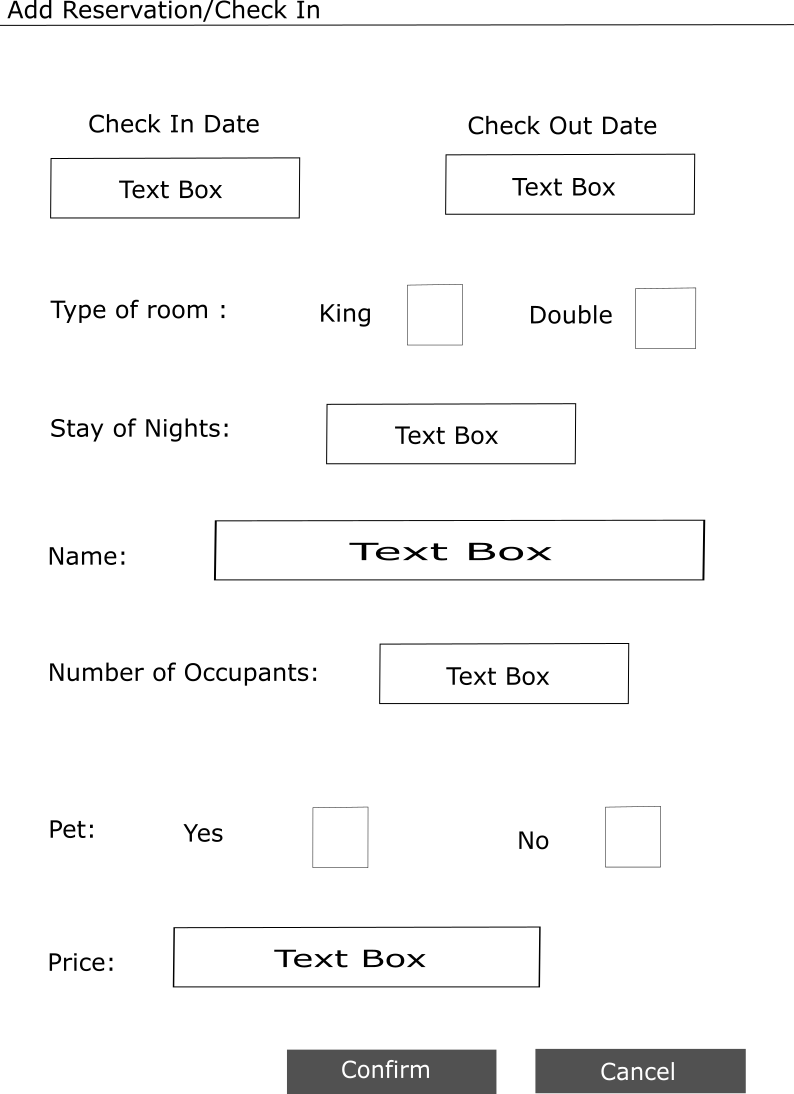
\includegraphics[height=250px, width=350px]{ResrvationGUI.png}
\caption{Reservation system}
\label{Interface}
\end{figure}


\section{Project Timeline}
Go back to your notes and look up a typical project development life cycle for the Waterfall approach.  How will you follow this life cycle over the remainder of this semester?  This will usually involve a chart showing your proposed timeline, with specific milestones plotted out.  Make sure you have deliverable dates from the course schedule listed, with a plan to meet them (NOTE: these are generally optimistic deadlines).

\section{Project Structure}
At first, this will be a little empty (it will need to be filled in by the time you turn in your final report).  This is your chance to discuss all of your design decisions (consider this the README's big brother).

\subsection{UML Outline}





\subsection{Design Patterns Used}
Make sure to actually use at least 2 design patterns from this class.  This is not normally part of such documentation, but largely just specific to this class -- I want to see you use the patterns!


\section{Results}
This section will start out a little vague, but it should grow as your project evolves.  With each deliverable you hand in, give me a final summary of where your project stands.  By the end, this should be a reflective section discussing how many of your original goals you managed to attain/how many desired use cases you implemented/how many extra features you added.

\subsection{Future Work}
Where are you going next with your project?
For early deliverable, what are your next steps?  (HINT: you will typically want to look back at your timeline and evaluate: did you meet your expected goals?  Are you ahead of schedule?  Did you decide to shift gears and implement a new feature?)
By the end, what do you plan on doing with this project?  Will you try to sell it?  Set it on fire?  Link to it on your resume and forget it exists?

\begin{thebibliography}{1}

\bibitem{IEEEhowto:kopka}
H.~Kopka and P.~W. Daly, \emph{A Guide to \LaTeX}, 3rd~ed.\hskip 1em plus
  0.5em minus 0.4em\relax Harlow, England: Addison-Wesley, 1999.

\end{thebibliography}



\begin{IEEEbiography}{Michael Shell}
Biography text here.
\end{IEEEbiography}

% if you will not have a photo at all:
\begin{IEEEbiographynophoto}{John Doe}
Biography text here.
\end{IEEEbiographynophoto}

\begin{IEEEbiographynophoto}{Jane Doe}
Biography text here.
\end{IEEEbiographynophoto}


\end{document}